\section{Tätigkeit in Magdeburg}

Wie erwartet war mein Kommen dem Magdeburger Schulamt Abt. Oberschulen willkommen, obwohl ich als ehemaliges Mitglied der \ac{nsdap} \enquote{politisch belastet} war. Von der sowjetischen Besatzungsmacht war ab sofort an allen öffentlichen Schulen Russisch als Pflicht- und Hauptfach eingeführt worden, doch selbst für die wenigen Gymnasien Magdeburgs standen nicht genügend wirklich qualifizierte Lehrer zur Verfügung -- für die Volksschulen musste erst im Jahre 1946 mit der Ausbildung von Fachlehrern des Russischen begonnen werden. Meine Russisch-Fakultas war also eine sehr begehrte Mangelware und ich verwaltete ab 29.11.45 eine Studienratsstelle am Domgymnasium.

Wenige Tage später übernahm ich noch in den Abendstunden den Latein- und Englischunterricht in den Abschlussklassen einer Privatschule, die auf das Abitur vorbereitete. Als ich einmal mit Staunen bemerkte, dass an der gleichen Schule nachmittags Stenographie- und Schreibmaschinenunterricht erteilt wurde, gab mir der geschäftstüchtige Chef die Erklärung: \enquote{Kleinvieh gibt auch Mist!}

Nachdem ich zunächst ein paar Tage bei dem Altphilologen Dr. Fischer neben dem Domgymnasium gewohnt hatte, bekam ich ein kleines Zimmer \marginpar{124} im Erdgeschoss bei dem Kinobesitzer Ostmann in der Nähe des Bismarck-Realgymnasiums, einem modernen Gebäude, in dem bald die Russen ihr Offiziersheim mit Schulungsräumen etc. installieren. Mein kleines Zimmer war nicht heizbar, ich durfte aber in manchen Stunden die warme Küche benutzen. So überstand ich einigermaßen die Zeit strengen Frostes, der bald im Dezember einsetzte. Für die Schulen gab es bis in den Januar 1946 kein Heizmaterial, die Temperatur sank in den Klassenräumen bis auf 0°, so dass ein normaler Unterricht unmöglich war: die Schüler erhielten Hausaufgaben, die in der Klasse kurz überprüft wurden. Einige Kollegen nahmen in einem geheizten Keller russ. Sprachunterricht bei mir, sie zahlten in ein paar Stücken Seife, einem Handtuch, Taschentüchern und sogar einem Nachthemd. Das einzige, was es noch zu kaufen gab, waren Bücher; von dieser Möglichkeit machte ich reichlich Gebrauch und tauschte u.a. bei einem 16-jährigen Jungen, der sich bei mir Rat und Hilfe bei seinen dichterischen Versuchen holte, eine große Dampfmaschine ein, ein willkommenes Weihnachtsgeschenk für meine beiden Jungen, die inzwischen (fast) 9 bzw. 7 Jahre alt geworden waren. Das Weihnachtsbäumchen konnten wir nur mit einer einzigen Kerze schmücken.

\marginpar{125} Meine Familie musste zunächst weiter in Treuenbrietzen bleiben, denn in Magdeburg, dessen ganze Innenstadt in einer schrecklichen Aprilnacht von 1000 Bombern in einen riesigen Trümmerhaufen verwandelt worden war, herrschte äußerster Wohnungsmangel. Der Schulbetrieb war auch in Treuenbrietzen, wo es keine höhere Schule gab, wieder in Gang gekommen, und die beiden Jungen besuchten eine Volksschule. Hier und da machte sich trotz der aus Schlesien und Pommern/Ostpreußen vertriebenen Kollegen ein starker Lehrermangel im sowjetisch besetzten Raum bemerkbar, da viele der früheren Parteigenossen, und deren Zahl war unter den Lehrern und Schulleitern beträchtlich, von den Sowjets verhaftet und entweder in die Sowjetunion oder in die deutschen Konzentrationslager verschleppt worden waren. Aus den in deutschen Lagern befindlichen und von deutschen Kommunisten bewachten Parteigenossen wurden nach Jahresfrist 60\% entlassen. Die übrigen 40\% waren, so hieß es, in ihrer 1-jährigen Haft \enquote{gestorben}. Sie kehrten nie zurück. Die Flüsterpropaganda wollte wissen, dass sie von deutschen Kommunisten zu Tode geprügelt oder an schlimmster Unterernährung zugrunde gegangen seien. Die lebend Davongekommenen hüteten sich davor, selbst in der eigenen Familie irgendetwas aus der Gefangenschaft zu erzählen. Die Furcht vor Denunzianten war groß -- und allzu begründet.

In der Schulverwaltung saßen selbstverständlich nur politisch \enquote{unbelastete} Männer und Frauen. Stadtschulrat war der Endfünfziger Linke, SPD, Oberschulrätin war die liberale Stud. Rätin Justen, die ihre antihitlerische Haltung durch Taten beweisen konnte. Lehrer, die nicht als Aktivisten, sondern nur als Mitläufer der \ac{nsdap} eingestuft wurden, ließ man in ihrem Amt. Im Schulbetrieb wurde alles \enquote{Nazistische} ausgemerzt, ein russischer Schuloffizier überwachte streng diese Säuberung, alles Militaristische verschwand. Als er in der Lehrerbücherei des Domgymnasiums ein französisches kleines Konversationslexikon entdeckte, war er ungehalten und ließ es entfernen, weil sich in ihm Bilder von (historischen) Soldaten und Uniformen befanden. Die Stoffpläne änderten sich -- abgesehen von Einführung des Russischunterrichts natürlich besonders in Geschichte und Gegenwartskunde, auch der Deutschunterricht wurde schrittweise im Sinne des Marxismus-Leninismus umgestaltet.

Weder in der Schulverwaltung noch in den Lehrerkollegien gab es Leute mit nennenswerten Kenntnissen der russischen Geschichte und Kulturgeschichte oder der Eigenart der russ. Menschen. So informierte sich Linke bei mir über \enquote{das, was man so im Umgang mit Russen wissen muss}. Sein Nachfolger im Amt begann sein ausgedehntes Gespräch mit mir mit den Worten, die Russen seien für ihn eine große Enttäuschung. Allerdings meinte einer seiner Kollegen, der ihn sehr gut kannte und dem ich davon erzählte, damit habe er mir eine Falle stellen wollen. Ich habe niemals ein Hehl daraus gemacht, dass ich der von den Russen arrangierten \enquote{Sozialistischen Einheitspartei SED} nicht beitreten werde.

\marginpar{127} Die Einführung der russischen Sprache auf der Oberstufe des Domgymnasiums in allen Klassen mit 6 Wochenstunden ging nicht ganz ohne Schwierigkeiten vor sich. Eine Oberprima -- gymn. -- hörte meine Ausführungen, die ich selbstverständlich möglichst interessant zu gestalten suchte, zwar diszipliniert zu, reagierte aber auf alle Lehrerfragen mit Schweigen. In der 4. Stunde verlangte ich eine Erklärung dieser Reaktion. Der Klassensprecher erklärte, man habe nichts gegen meine Person oder die Unterrichtsweise, die im Gegenteil durchaus gefalle, die Klasse lehne es aber geschlossen ab, diese Sprache zu erlernen. Ich nahm es zur Kenntnis und unterrichtete einfach weiter, wobei ich noch mehr als bisher alle Register zog, um Interesse für russische Sprache und Kultur zu erwecken.

Ich teilte jedoch dem Schulleiter, \ac{ostd} Weitz diesen Vorfall mit. Der war aufgebracht, wollte sofort das Schulamt und \enquote{die Russen} informieren. Es gelang mir schließlich ihn von seinem Vorhaben abzubringen mit der Versicherung, ich werde die Angelegenheit selbst bereinigen. Das gelang mir auch: als ich in der nächsten Stunde einzelne aufrief, sah ich, wie ihnen ermunternd aus der Klasse zugenickt wurde und das Eis war gebrochen.

Diese Klasse arbeitete bis auf zwei Schüler sehr gut mit, so dass sie nach Jahresablauf in der Reifeprüfung gute Grundkenntnisse aufweisen konnte.

Nicht ganz unwesentlich bei diesem Erfolg \marginpar{128} war der Umstand, dass dieser Klasse die logisch-grammatische Schulung in Latein- und Griechischunterricht bei der Erlernung einer weiteren indogermanischen und ausgesprochen synthetischen Sprache sehr zustatten kam.

Mitte Januar wurde ich zum Stellvertretenden Kommandanten von Magdeburg, dem Major Sikiejew, beordert. Wie ich hörte, waren auch einige andere Magdeburger Pädagogen bestellt worden, die über russische Sprachkenntnisse verfügten. Er suchte zwei Lehrkräfte, die dem russ. Offizierskorps Unterricht in der deutschen Sprache erteilen sollten. Major S. war etwa 35-40 Jahre alt und machte einen intelligenten und, wie sich im Gespräch herausstellte, gebildeten Eindruck. Nach einigen Fragen über meine Lehrbefähigungen und berufliche Arbeit unterhielten wir uns über die russische Literatur, wobei er Gorkij und die Zeit nach 1918 ausklammerte. Er merkte, dass ich gute literarische Kenntnisse hatte und sie schätzte, und wir sprachen etwas eingehender über L. N. Tolstoj. Ich gefiel ihm anscheinend und er fragte mich, welchen Preis ich für die Doppelstunde, also 1,5 Zeitstunden, wünsche. Ich verlangte, nicht schüchtern, 20 Mark. Er meinte, das sei viel Geld, aber er willige ein, wenn ich gute Arbeit leiste. Später erfuhr ich, dass die anderen Bewerber bescheiden nur 5~M verlangt hatten. Ich fragte nun zum Abschluss, ob er denn keine andere Frage habe (ich dachte an das heikle Thema meiner politischen \marginpar{129} Vergangenheit), worauf er festen Blickes und betont antwortete: \enquote{Ich \underline{will} keine weiteren Fragen stellen.}

Außer auf mich fiel die Wahl noch auf einen ostpreußischen Studienrat, der jedoch auf die Dauer den Russen wenig gefiel, überdies erkrankte und nach knapp zwei Jahren an durch Unterernährung hervorgerufener Tbc starb.

Ich hatte etwa 20 Sowjetoffiziere an zwei Vormittagen zu unterrichten, was für mich interessant und förderlich war, da ich den ganzen grammatischen Unterricht in russischer Sprache zu führen hatte -- und erholsam dazu: sie kamen unfreiwillig und hatten wenig Lust die Sprache des besiegten und in jahrelanger Schulung abschätzig behandelten Volkes zu lernen; war die Luft rein und kein Vorgesetzter zu erwarten, so zogen sie es vor, in Nebenräumen Billard u.a. zu spielen und ich saß meine Zeit lesend oder mit Russen, z.B. der Dolmetscherin, plaudernd ab. Zweimal im Jahr 1946 hospitierte mich Major Sikiew an, beim zweiten Besuch forderte er mich eingangs auf, den Unterricht eine Stunde lang ohne Buch zu erteilen. Er war beide Male zufrieden. Unangenehm war, dass man mich bespitzelte: einer meiner Primaner wurde zu den Russen bestellt, zwei Tage festgehalten und vernommen; worum es sich handelte, konnte man bei den sowjetischen Methoden wegen des strengen Schweigebefehls, der den Betroffenen bei der Entlassung erteilt wurde, nie erfahren. Als ich einmal im Unterricht einen Offizier den Satz \enquote{ich lese die Zeitung} konjugieren ließ, tat er so: ich lese die Pravda, du liest den Völkischen Beobachter\footnote{der Völkischer Beobachter war die Parteizeitung der \ac{nsdap}}. \marginpar{130} Ich hatte einmal in einer Oberprima ein paar Worte über die sakrale russische Architektur gesprochen und dabei geäußert \enquote{Der Vassilij Blazenuij\footnote{Bezeichnung für die weltberühmte \enquote{Basilius-Kathedrale} am Roten Platz in Moskau} ist wirklich schön.} 14 Tage später kam aus Offiziersmunde die Antwort: \enquote{Schön wie der Wassilij Blazenuij}\dots

Die deutsche Magdeburger Dolmetscherschule wurde wieder aufgemacht, zunächst nur mit Russisch als Lehrfach, das vorwiegend von Deutschrussinnen erteilt wurde, vor allem von einer gewissen Frau Brossart, die sich später als üble Denunziantin entpuppte. Ich übernahm als einzige pädagogisch ausgebildete Fachkraft eine Fortgeschittenen-Klasse. Die gesamte Verwaltungsarbeit leistete im übrigen Dr. Lechner, der frühere Direktor der Victoria Oberschule, der als ehemaliger \ac{pg} nun als Sekretär beschäftigt wurde.

Wenn ich noch im Laufe des Winters in der zu schwachem Leben erweckten Volkshochschule einen Einführungslehrgang in die russische Sprache für Erwachsene übernahm, so trieb mich dazu nicht etwa beruflicher Ehrgeiz, sondern der Zwang, eine siebenköpfige Familie zu ernähren. Frau und Kinder erhielten die Lebensmittelkarte No 5 (siehe Anhang \ref{tab:lebensmittelkarten}), die sogenannte \enquote{Friedhofskarte}, deren Namen alles besagt. Lehrer bekamen Karte 4, die mich als mittelstarken Esser bei weitem nicht sättigen, obwohl ich in den ersten Magdeburger Monaten mittags im Ratskeller eine nicht billige markenfreie Kartoffelsuppe mit Gemüse (Porree, Mohrrüben etc.) zu mir nehmen konnte und abends von meinen Wirtsleuten eine warme, allerdings nicht sehr gehaltvolle Suppe erhielt. Im Februar pflegte ich in der Nacht vor Hunger aufzuwachen, den ich nicht zu stillen vermochte, \marginpar{131} bis ich einen Bäcker in der Leibnitzstraße fand, der mir unter dem Ladentisch ab und zu ein markenfreies Brot, natürlich zum vielfachen Preis, verkaufte. Leider versiegte diese Quelle nach ein paar Monaten: der Bäcker konnte bei einer Kontrolle den Verbleib von mehreren Zentnern Mehl nicht nachweisen und wurde eingesperrt, der Laden geschlossen.

Immerhin war es mir möglich, bei meinem etwa monatlichen Besuchen in Treuenbrietzen meiner Familie ein- oder zweimal einen Brotkanten mitzubringen, den ich mir abgespart hatte. Als ich Pfingsten 1946 unsere Jüngste, Ulla, knapp 2,5-jährig bei der Hand nahm um mit ihr spazieren zu gehen, schüttelte sie traurig den Kopf und sagte: \enquote{nich pazieren gehn, wima eine Nitte} (lieber eine Schnitte essen) -- und ich war mit leeren Händen gekommen!\footnote{Anm. Helga: das trug sich an einem Nachmittag im Hof der \enquote{bösen} Frau Ahlborg zu. Ich kann mich noch gut an die runden Holzstämme erinnern, die dort aufgehäuft lagen. Ullas Antwort war für Vati eine höchst schmerzliche Antwort, die er sein Leben lang nicht vergessen konnte und die er uns oft erzählte.}

Mein Tischgenosse im Magdeburger Ratskeller war übrigens der Intendant des Magdeburger Stadttheaters, dem ich u.a. Anregungen für die Regie von Schulaufführungen verdanke.

In den Jahren 1945/46 suchten russ. Offiziere der Besatzungsarmee -- wohl illegal -- in den Besitz von Autos zu kommen [zum Preis von] mehrmonatlichen Gehältern. Wahrscheinlich spielte hierbei die GPU\footnote{GPU: seit 1922 die Geheimpolizei der SU} die Hauptrolle vielleicht auch [nur] als Vermittlerin. Man verhaftete \enquote{Kapitalisten}, ehemalige \ac{pg} oder auch nur \ac{vg}, die ein Auto besaßen und setzte sie mehrere Tage unter Druck, bis sie sich bereit erklärten, den Russen ihr Auto \enquote{zu verkaufen}. Mein Hauswirt, der clevere Kinobesitzer Ortmann, war jedoch den Russen gewachsen in einer Szene, die sich vor meiner Zimmertür und vor meinen Augen abspielte. Einem Russenauto entstiegen ein Offizier und eine Dolmetscherin, die nach Herrn Ortmann fragten, der auch sofort erschien. Man erklärte ihn für verhaftet und forderte ihn auf, den beiden zum Auto zu folgen. Herr Ortmann brach unmittelbar vor der Entreetür zusammen, blieb starr mit geschlossenen Augen liegen, das Gesicht hochrot, er atmete schwer, alle Versuche, den schweren, starr daliegenden, anscheinend bewusstlosen Mann aufzurichten, blieben vergeblich. War es ein epileptischer Anfall oder ein Herzkollaps? Nur ein Arzt hätte die Frage beantworten können. Ich wurde gefragt -- die Dolmetscherin erkannte mich als Dozent des Offizierkorps -- ob Ortmann schon einmal einen solcher Anfälle gehabt habe, und ich antwortete ausweichend, ich wisse, dass er herzkrank sei. -- Ratlosigkeit der beiden Russen -- dann verließ man achselzuckend die Wohnung und fuhr mit dem Auto ab. Die Russen kamen übrigens nicht wieder. Als die Luft rein war, normalisierte sich Ortmanns Zustand rasch. Ich vermute, dass er diese Szene mit einem Arzt gegen gute Bezahlung einstudiert hatte. Ortmann protzte mit seinem Gelde; als ich ihn einmal nach einem früher wirklich guten Magdeburger Lokal fragte, nannte er eines, in dem er zu verkehren pflegte, fügte aber hinzu, für mich wäre es natürlich nichts gewesen, da in diesem Lokal nur Personen mit einem Jahreseinkommen von über \num{100000} Goldmark verkehrten\dots

Die schulischen Sommerferien (Ende Juli -- Anfang August) wurden wegen des großen Nachholbedarfs in diesem Sektor von der Besatzungsmacht auf knapp 14 Tage verkürzt. In dieser Zeit fanden in der Brüdergemeinde Gnadau, etwa \marginpar{132} 12~km von Magdeburg in der Börde gelegen, in der dortigen Jungenoberschule mit Internat ein pädagogisches Seminar für Studienräte unter Leitung der Oberschulrätin Justus statt, zu dem auch ich eingeladen war. Einen gewissen Anreiz bot schließlich auch der von der Besatzungsmacht für die Teilnehmer bewilligte Verpflegungszuschuss. Man wurde tatsächlich bei den Mahlzeiten fast satt. Die sympathische herrenhuter Atmosphäre hatte ich schon als Schüler in Gnadenberg bei Bunzlau kennen gelernt. Zudem waren meine Mutter und Großmutter in einer herrenhuter \enquote{Töchterschule} in Kleinwelka bei Bautzen erzogen worden und hatten dort eine für die damalige Zeit gute Allgemeinbildung mit soliden Kenntnissen der französischen und englischen Sprache erworben und waren mit Plus- und Minusseite mit herrenhuter Geist imprägniert.\footnote{Anm. Helga: Die \enquote{Herrenhuter Brüdergemeinde} waren eine christliche Gemeinschaft, bei denen die Prüfung des eigenen Gewissens Teil der Erziehung war. \enquote{Bleib bei der Wahrheit} und \enquote{prüfe dein Gewissen} waren von Vati gern geäußerte Aufforderungen bzw. Ermahnungen, die er von seiner Mutter übernommen hatte und die vermutlich aus dieser Erziehung stammten\dots} Dort begegnete ich einem Kostudenten aus der Breslauer Vorkriegszeit, der sich wie ich auch, in der \enquote{Freien Bruderschaft} betätigt hatte. Er war Leiter der Gnadauer Oberschule und half mir in dieser Eigenschaft in den bevorstehenden Notjahren bei der Erziehung unserer beiden Jungen, indem er sie in sein Internat aufnahm.

Die Familie Sternberg wurde 1946 von einem schweren Schicksalsschlag getroffen: der einzige schon erwachsene Sohn, Jurastudent, der einer antisowjetischen Untergrundbewegung angehörte, wurde von Deutschen denunziert und verschwand in sowjetischer Haft. Schon nach 14 Tagen erhielten die Eltern die Nachricht, \marginpar{134} ihr Sohn sei in der Haftanstalt gestorben. Es gehört viel Höllenphantasie dazu, um sich die Qualen in der stalinistischen Haftanstalt vorzustellen, die seinem Tod vorausgingen.

Im Seminar gab es übrigens nützlichen Gedankenaustausch und einige Anregungen, die Atmosphäre war noch ziemlich frei von Marxismus-Leninismus.\\

In der Mittagspause und am Abend ging ich mit einigen anderen Teilnehmern ährenlesen und war stolz, beim nächsten Besuch in Treuenbrietzen 3 Pfund Roggenkörner mitbringen zu können.

Meine Bemühungen um eine Wohnung blieb ohne Erfolg. So wollte ich mich mit Margots Zustimmung zunächst mit einem Wochenendhaus begnügen. Es gab eine große Laubenkolonie unmittelbar am Stadtrande. Der Vorsteher dieser Kolonie war ein Kommunist, der zwar unter Hitler sein Schwarzhemd mit dem Braunhemd vertauscht und sogar einen kleinen Funktionärsposten innegehabt hatte, aber es gelang ihm glaubhaft zu machen, dass er nur zu \enquote{Studienzwecken} in die \ac{nsdap} eingetreten sei. Bei meinem Besuch beeindruckte ihn meine Beziehung zu den Russen, so dass er mir sofort ein brauchbares \marginpar{135} Angebot machte. Bevor ich den Mietvertrag abschloss, erfuhr ich aus mehreren Quellen, dass diese Wochenendhäuser das häufige Ziel nächtlicher \enquote{Besuche} und Plünderungen durch russische Soldaten seien, wogegen man sich nicht wirksam wehren könne. Unter diesen Umständen trat ich zurück.

Um von dem Papiergeld, das wir durch Verkauf von Stücken der Wohnungseinrichtung in Bad Salzbrunn gewonnen hatten, einen Teil halbwegs \enquote{wertbeständig} anzulegen, kaufte ich Briefmarken und lernte auf diese Weise die Frau eines in amerikanische Gefangenschaft geratenen Mittelschullehrers kennen, die in der Stehr'schen Buchhandlung in der Hegelstraße / Ecke Tauentzienstraße eine kleine Briefmarkenhandlung eingerichtet hatte. Sie wohnte im 2. Stock des sogenannten Rektorenhaus Leibnitzstraße 30, als Untermieterin des pensionierten Konrektor Schultze. Anfang August erhielt sie die Nachricht, dass ihr Mann demnächst aus der Gefangenschaft zurückkehre und dass ich dann in ihre 3-Zimmer Mietswohnung einziehen könne. Ich erhielt die behördliche Genehmigung und in der ersten Septemberhälfte fuhr unsere Familie auf einem offenen Laster mit unserem dürftigen, armseligen Hausrat in etwa 5 Stunden von Treuenbrietzen nach Magdeburg. Wir brachten in die neue 3-Zimmerwohnung -- das mittlere Zimmer war kaum 12 qm groß -- kaum mehr als eiserne Bettstellen mit schlechten Matratzen, ein paar Federbetten mit, es fehlten vor allem Tische und Stühle, die wir zunächst durch Kisten ersetzten. Als erstes kauften wir in Magdeburg ein Federbett für 2 Pfund Kaffee, den wir für 500 Mark pro Pfund erstanden hatten. Als Studienrat (die Beförderung zum \ac{ostr} wurde nicht anerkannt) erhielt ich monatlich 700 Mark brutto, wovon jedoch 50\% als Strafe für meinen Eintritt in die \ac{nsdap} abgezogen wurden, sodass mir nur ca. 340~M ausgezahlt wurden für die 6-köpfige Familie.

Es vergingen Monate und Jahre, bis wir unsere Behausung -- die im Bombenhagel zerstörten Fensterscheiben waren durch milchige Plastikscheiben\footnote{Anm. Helga: es handelte sich hierbei um dünne Platten aus \enquote{Igelit}, einem Weich-PVC. Igelit wurde bei Kälte spröde, darum gingen die Fenster im Winter leicht kaputt} ersetzt worden -- durch Kauf oder leihweise erhaltene Möbelstücke einigermaßen erträglich eingerichtet hatten.

Unter uns im 1. Stock wohnte Herr Milleville, Direktor einer Sonderschule, mit seiner Frau. Mit ihnen unterhielten wir in unserer ganzen Magdeburger Zeit freundschaftliche Beziehungen.

Unsere beiden Jungen besuchten zunächst die Leibnizschule, eine solide Volksschule; sie rannten die 50 Schritte über den Schulhof, der ihnen außerhalb der Unterrichtszeiten als Spielplatz diente.

Der Winter 1946/47 war sehr streng, wir froren in der Wohnung; abends, wenn die Kinder zu Bett gebracht waren, saß ich oft mit Margot auf der Ofenbank, den Rücken fest an den nur lauwarmen, unzureichend mit Braunkohlengrus\footnote{Grus = fein zerbröckelte Kohle, grobkörniger Kohlenstaub} geheizten Ofen gelehnt. Auch alle Schularten wurden nur unzureichend geheizt, sodass der Unterricht gekürzt wurde oder auch ganz ausfiel. Warm hatten es \marginpar{136} nur die Russen, bei denen ich noch zusätzlich an zwei Wochenabenden je zwei Stunden Französisch und Englisch unterrichtete. Unsere äußerst unzulängliche Ernährung -- waren wir doch ausschließlich auf die Lebensmittelkarten angewiesen -- wurde in der lange Frostperiode besonders spür- und sichtbar, sodass man mir auf Anweisung der Russen die Lebensmittelkarte 2 bewilligte. Der Frost war so streng, dass die Elbe im Februar einen dicken Eispanzer trug, zur Freude unserer Kinder, die vermummt bei -15° über die Elbe zur Werderinsel gehen konnten.\footnote{Anm. Helga: Die Kinder waren die Brüder Wolfgang und Harald. Wir Mädchen, Ulla 3, Helga knapp 5 waren zu klein für solche \enquote{Ausflüge} und ohne das entsprechende Schuhwerk! Ich kann mich aber erinnern, dass die Jungen im Winter in der Elbe treibenden Eisschollen betreten haben, wir Mädchen durften davon aber zu Hause auf keinen Fall erzählen.}

Margot holte in dieser Kälte mit dem Handwagen in Abständen einen Zentner Brennmaterial bestehend aus minderwertigen Braunkohlegrus mit dem wir das mittlere \enquote{Wohnzimmer} ein wenig anwärmen konnten. Wochenlang vermieden wir uns auszuziehen\dots und zu waschen.\footnote{Anm. Helga: In der Wohnung gab es nur eine Toilette für uns zwei Mietparteien (8 Personen) und kein Badezimmer. Die Toilette war so groß, dass man im Sitzen gerade noch die Tür schließen konnte. Nachttöpfe waren üblich, auch bei den Erwachsenen. Jeden Morgen leerte Margot die Nachttöpfe in der Kloschüssel aus. Es gab auf der Toilette ein kleines Handwaschbecken. Wenn man sich waschen wollte, nahm man das Wasser von dort in einer Waschschüssel mit in die Wohnung}

Auf den strengen Winter folgte ein heißer, trockener Sommer; schon im Mai verblasste das Wiesengrün auf der Werderinsel und ich sammelte nur mit großer Mühe hier und da im Schatten der Bäume und Sträucher einiges Wildgemüse wie Melde und Sauerampfer, das wir so dringend für unsere vitaminarme Ernährung brauchten. Bald gab es keine Kartoffeln mehr, wir beneideten die glücklichen Einheimischen, die vielfach in ihren Kellern noch Vorräte dieser kostbaren Knollen besaßen. Die Hungertuberkulose fürchtend, der damals viele Magdeburger, jung und alt zum Opfer fielen -- \marginpar{137} allein von meinen Primanern erlagen sieben dieser Mangelkrankheit -- stellte ich in den Monaten August und September jede Nebentätigkeit nachmittags und abends ein und lag, jeden körperlichen Kraftverschleiß meidend, den ganzen Nachmittag lesend und schreibend auf meinem Nachtlager.

Im Herbst arbeitete Margot mit Hiltrud Buttkus, der Frau eines Magdeburger Archivars, die sie beim Anstehen vor einem Geschäft kennengelernt hatte\footnote{Anm. Helga: Hiltrud blieb lebenslang eine enge Freundin meiner Mutter} im Akkord bei Bauern auf Kartoffelfeldern. Als Bezahlung erhielten sie ein paar Zentner Kartoffeln und Zuckerrüben. Diese ungewohnte schwere Arbeit führte bei Margot zu einer Überanstrengung, die leider eine dauernde Schädigung ihrer Gesundheit zur Folge hatte.

Die Zuckerrüben wurden tags von Margot und Hiltrud B. geschnitten und gekocht und nachts wurde im Keller der Rübensaft eingekocht, wobei ich mich mit Herrn Buttkus im Umrühren ablöste. Unserer Ernährung kam ein weiterer Umstand zugute: einzelne Offiziere oder deren Kinder nahmen bei mir Privatstunden, für die ich in Lebensmitteln entlohnt wurde. Ich erhielt für die Stunde 100 gr Speck, gelegentlich auch Fleisch und deformierte Kommissbrote\footnote{Anm. Helga: Kommissbrot ist ein einfaches, haltbares Brot zur Versorgung von Soldaten. In meiner Familie herrschte großer Jubel, wenn er mit einem Rucksack solcher Brote, manchmal sogar mit etwas Fleisch, heimkehrte}, die die Russen nicht essen mochten.

Meine schulische Tätigkeit wurde mit Beginn des Winterhalbjahres umfangreicher: In der neu gegründeten Lehrerbildungsanstalt übernahm ich mehrere Lehrgänge der russischen Sprache. Die Lehreranwärter im Alter von 17 bis 35 Jahren hatten eine sehr unterschiedliche Vorbildung, großenteils war ihnen geistige Arbeit fremd, so dass für sie die Erlernung einer Fremdsprache, besonders einer synthetischen, flexionreichen Sprache wie des Russischen, oft mit großen Schwierigkeiten verbunden war. Viele von ihnen unterrichteten vormittags in Volksschulen: sie gaben das, was sie am Nachmittag vorher gelernt hatten, an ihre Schüler weiter. Ich erinnere mich an einen Leitartikel im kommunistischen \enquote{Magdeburger Tageblatt}, \marginpar{138} in dem dieses Verfahren als geradezu ideal gepriesen wurde. In welche Verlegenheit der frischgebackene \enquote{Lehrer} durch wissbegierige und intelligente Schüler gebracht wurde, kann man sich lebhaft vorstellen.

Im Deutschlehrbuch eines 16-jährigen russ. Privatschüler entdeckte ich ein langes deutschsprachiges Gedicht von Johannes R. Becher, das eine einzige Beschimpfung und Beschmutzung der deutschen Soldaten war, wohlgemerkt nicht etwa der SA oder SS, was noch verständlich von einem deutschen Antifaschisten gewesen wäre. Ich las es gegen Ende einer Russischstunde in einer Prima vor. Das Urteil der Klasse: \enquote{der Verfasser ist ein Schweinehund!!} Missbilligung vortäuschend erwiderte ich: \enquote{Ich will nichts gehört haben. Der Verfasser ist der Präsident der deutschen Dichterakademie!} Die ganze Klasse: \enquote{Dann ist er erst recht ein Schweinehund!}

Zur Erläuterung: in den ersten Jahren nach der deutschen Katastrophe hatte ich die Gewähr, dass in den oberen Klassen des Domgymnasiums noch keine SED-infizierten Schüler saßen. Zwischen den Schülern und mir bestand ein festes Vertrauensverhältnis, sie verstanden, dass ich (gelegentlich) den Schein waren musste\dots

Der Leiter der Magdeburger Lehrerbildungsanstalt, ein wirklich gebildeter maßvoller Mann aus der alten Schule, mit dem man gern zusammenarbeitete, wurde alsbald durch einen Parteikommunisten namens Biemüller ersetzt, der den Titel \enquote{Oberregierungsrat} führte -- in den allerersten Jahren behielt das neue Regime die alten Titel bei -- ein äußerst fragwürdiger (gelinde ausgedrückt) Charakter. Er setzte in seiner Eigenschaft als Parteifunktionär die Witwe eines im kommunistischen Konzentrationslager gestorbenen nationalsozialistischen Kollegen so unter Druck, dass sie ihm zitternd ihre schöne Wohnungseinrichtung für ein Butterbrot verkaufte\dots In seinem Amtszimmer hängte er sofort nach Erscheinen im Jahre 1948, die Karte des neuen Polens auf, mit der de facto Oder-Neiße Grenze. Er pries die Grenze als schön und gerecht und fragte mich nach meiner Meinung, offenbar um mir, einem aus dem Osten Vertriebenen, ein Bein zu stellen. Ich antwortete \enquote{Pan juz mówisz popolsku?} (Sie sprechen schon polnisch?) Er darauf: \enquote{Vielleicht haben Sie mich gefragt ob ich polnisch spreche?} Ich bejahte. Er: \enquote{Nein, leider kann ich diese Sprache noch nicht.} Damit war ein Gespräch beendet, mit dem Biemüller nicht viel anfangen konnte.

In der Straßenbahn begegneten wir 1947 Frau Dr. Else Noack, Margots einstiger Lehrerin in der Breslauer Sozialen Frauenschule, die damals unter der Leitung von Frau Dr. Besser gestanden hatte. Die Leitung der 1946 wieder eröffneten Magdeburger Sozialen Frauenschule übertrug man Dr. Noack. Mit ihr verband uns bald eine Freundschaft, die sich jahrzehntelang bis zu ihrem Tode im Jahre 1976 bewähren sollte.

Im gleichen Jahr 1947 wurde ich \enquote{entnazifiziert}. Die über 300 im Lehrberuf tätigen \marginpar{140} ehemaligen Mitglieder der \ac{nsdap} der Kreise Magdeburg und Schönebeck, die den 2. Weltkrieg und die erste Zeit der russischen Besatzung lebend überstanden hatten, wurden im Schulamt von einer 11-köpfigen Kommission verhört, bestehend aus antifaschistischen Vertretern der Parteien und der Schulbehörde. Alle belasteten Lehrkräfte wurden \enquote{entnazifiziert}, d.h. für den Lehrberuf im SED-Staat tragbar erklärt, mit zwei Ausnahmen, von denen ich eine war.

Ich erhielt jedoch einige Tage später die Nachricht, dass meine Überprüfung durch diese Kommission wiederholt werden sollte.

Bevor das zweite Verhör begann, nahmen mich der Stadtschulrat Linke und Schulrat Nolte ins Gebet, ich dürfe unter keinen Umständen erneut aussagen, dass ich 1933 an die Führungsqualitäten und den Willen Hitlers geglaubt habe, Deutschlands politischen und wirtschaftlichen Schwierigkeiten zu überwinden und einen gerechten Sozialstaat zu schaffen. Daraus habe die Mehrheit der Kommission die Schlussfolgerung gezogen, dass ich ein echter Nazi sei. Ich befolgte also die Ratschläge der beiden Schulräte und betonte u.a. die Tatsache, dass ich mich zum linken sozialen Flügel der \ac{nsdap} unter Gregor Strasser rechnete, der schon 1934 von der SS ermordet wurde. Nun wurde ich tatsächlich entnazifiziert. Der Direktor der Dolmetscherschule der der Kommission angehörte, hatte u.a. wörtlich erklärt: \enquote{Wenn von den 300 ehemaligen \ac{pg} ein einziger die Wahrheit gesagt hat, dann war es Busse.} Wie ich erfuhr, waren zahlreiche \enquote{Angeklagte} entnazifiziert worden, die z.B. aussagten, den Antrag auf Aufnahme in die \ac{nsdap} in halb oder völlig trunkenem Zustande unterschrieben und schon am nächsten Morgen diesen Schritt bereut zu haben, jedoch an einem Widerruf durch die ängstliche Ehepartnerin gehindert worden zu sein.

Die Magdeburger Stadtbibliothek, die von den Russen zum größten Teil geräubert und nach der Sowjetunion verfrachtet worden war, wurde mit ihrem restlichen Bestand von nur \num{40000} Büchern wieder zur öffentlichen Benutzung freigegeben. In ihr entdeckte ich einige slawistische Werke, die ich im Frühjahr 1948, sobald im Lesesaal die Temperatur auf etwa 12° gestiegen war, stundenweise für meine Arbeiten benutzte.

Im Sommer 1948 fand in Berlin die erste Arbeitstagung der Russisch-Do\-zen\-ten bzw. Ausbilder der Russischlehrer in der sowjetischen Besatzungszone statt unter Leitung von Prof. Dr. Dembowski, einem leider schlechten Organisator. Ich hatte ein Referat aus dem Grenzgebiet von Russistik und Methodik des Russischunterrichts übernommen. An das Referat eines Berliner Professors der Slawistik über die Wechselbeziehungen zwischen der deutschen und russischen Literatur, das erhebliche Lücken und Mängel erhielt, schloss ich eine sich über 50 Minuten erstreckende \marginpar{142} Kritik, die er mir noch nach Jahren nicht vergessen konnte, da sie so \enquote{streng} gewesen sei. Hauptdiskussionsredner waren Dr. Müller-Schotte (Magdeburg) und ich -- zum Verdruss einiger junger Dozenten, die jedoch, wie sich zeigte, nichts Nennenswertes zu sagen hatten. Eine 3/4 Russin hielt streng nach der direkten Methode eine russische Grammatikstunde bei etwa 11-jährigen Mädchen, die äußerlich einen guten lebendigen Eindruck machte. Als Müller-Schott und ich jedoch anschließend Fragen an die Klasse richten durften, stellte sich heraus, dass so gut wie niemand aus der Klasse das Neudurchgenommene verstanden hatte.

Vor der Rückfahrt nach Magdeburg kaufte ich auf dem Schwarzen Markt am Bahnhof Friedrichstraße 2 Brote für 30 Mark.

Im Sommer 1948 besserte sich der Kaloriengehalt der Verpflegung unserer Familie nicht ganz unbeträchtlich. Und das kam so: In einer meiner Russischklassen befand sich ein annähernd 40-jähriger \enquote{verdienter Altkommunist}, von dem mir der schon erwähnte charakterlich höchst fragwürdige Chef der Lehrerbildungsanstalt, Biemüller, beizeiten sagte, er müsse unbedingt die Lehrerprüfung mit mindestens \enquote{gut} bestehen. \marginpar{143} Ich erwiderte ihm, dass dies in Russisch schlechterdings unmöglich sei, da er überhaupt nicht abstrakt denken könne und somit für ihn schon die Unterscheidung von Subjekt und Objekt geschweige denn der russischen Casus wie Instrumentalis und Lokativ unüberwindliche Hürden darstelle. Biemüller meinte, ich solle ihm Privatstunden geben, er könne mit einem wichtigen Lebensmittel zahlen. Und so geschah es auch: mein neuer Privatschüler, wohnhaft in einem großen Dorfe unweit Magdeburg, hatte einen Schwager, der in einer Ölmühle arbeitete und für seine engsten Freunde regelmäßig von der heißbegehrten Flüssigkeit einiges beiseite schaffte. Schon zu Beginn der 2. Stunde zog mein Kommunist ein Fläschchen aus der Rocktasche, damit meine Frau, wie er sagte, für die Kinderlein Kartoffelpuffer backen könne\footnote{Anm. Helga: An die Mahlzeiten mit dem Sonnenblumenöl kann ich mich sehr lebhaft erinnern: zum Essen legten wir unter den hinteren Tellerrand etwas unter, so dass das Öl im vorderen Teil des Tellers eine kleine \enquote{Pfütze} bildete. Nun tunkten wir die Brotstücke in das Öl und aßen es mit Genuss\dots
	
	In der Küche war eine große altmodische \enquote{Kochmaschine}, die aber nicht benutzt wurde. Wir benutzten tagsüber den 2-flammigen Gaskocher, der Eigentum von Frau Schulze war. Abends zog Frau S. ihren Kocher vom Gasanschluss ab und verschwand mit ihm in ihrem Zimmer, so dass meine Mutter dann nicht mehr kochen konnte. Nach einiger Zeit gelang es meiner Mutter, über Hiltrud Buttkus einen weiteren Gaskocher zu organisieren. Wieder zog Frau S. abends mit ihrem Kocher ab, aber meine Mutter holte nun ihren Gaskocher und konnte jetzt auch Abends kochen. Wie groß war am nächsten Morgen die Überraschung bei Frau S., als an \enquote{ihrer} Kochstelle bereits ein anderer Gaskocher stand\dots}. Später merkte ich, dass er auch Biemüller und die andern ihn unterrichtenden Dozenten \enquote{ölte}, um den Erfolg der Prüfung sicherzustellen. So kam es, dass das ganze Dozentenzimmer nach Öl roch und er schließlich die Lehrerprüfung \enquote{zusammengefasst} mit gut bestand; aus dem Rahmen fiel allerdings Russisch, da er nach wie vor mit der russischen Elementargrammatik auf Kriegsfuß stand, und ihn in der mündlichen Prüfung nur sein relativ gutes Gedächtnis für russische Gedichte rettete, so dass man auf \enquote{genügend} erkannte.

Der Ölmann besaß übrigens Humor. Er erzählte mir, sein Nachbar, ein Mann in den Dreißigern, arbeitete überhaupt nicht. Für ihn arbeite ein \marginpar{144} Huhn. Dieses Huhn lege täglich ein Ei, mit dem er auf den Schwarzen Markt gehe und es dort für 12~M (das war damals tatsächlich der Preis) verkaufe. Sein Huhn erarbeite ihm somit monatlich 360~M, eine Summe, die ihn für seinen Lebensunterhalt genüge.

Im Schulbetrieb gab es bald grundlegende Umwälzungen. Doch auch an schnurrigen Einfällen fehlte es den Russen in Karlshorst nicht, die das Schulschiff steuerten. Eine intensive Friedenspropaganda setzte ein, die Sowjetunion war die große Friedensmacht, während die Westmächte und bald auch die Bundesrepublik Deutschland der Kriegstreiberei bzw. des Revanchismus verdächtigt wurden. Die Friedenstaube von Picasso als Symbol wurde in zahllosen Millionen von Exemplaren gedruckt, die Schüler -- besonders der Volksschulen -- \enquote{spontan} dazu angehalten, sie an die Fensterscheiben der Klassenzimmer zu kleben. Diejenigen Klassen und Schulen, deren Fenster fast so dicht mit diesen Picasso Vögeln beklebt waren, dass die Sonnenstrahlen nur noch mit Mühe in die Schulräume dringen konnten, wurden öffentlich belobigt. Bald darauf hatte man einen neuen Gedanken: In allen öffentlichen Gebäuden wurden sogenannte \enquote{Friedensecken}, man könnte sie auch Altäre nennen, angelegt, in deren \marginpar{145} Mitte eine Lenin-, Marx-Engels- und vor allem natürlich Stalinbüste oder wenigstens ein entsprechendes Bild eines dieser in den Rang der größten Friedensapostel der Weltgeschichte beförderten Männer. Auch in unserem \enquote{Rektorenhaus} wurde im Treppenpodest zum 1. Stock eine Friedensecke mit einem Leninbild hergerichtet, in der sich zum Ärger des Schulwarts Fricke dessen Hund völlig respektlos zu benehmen pflegte.

\begin{figure}[t]
	\fbox{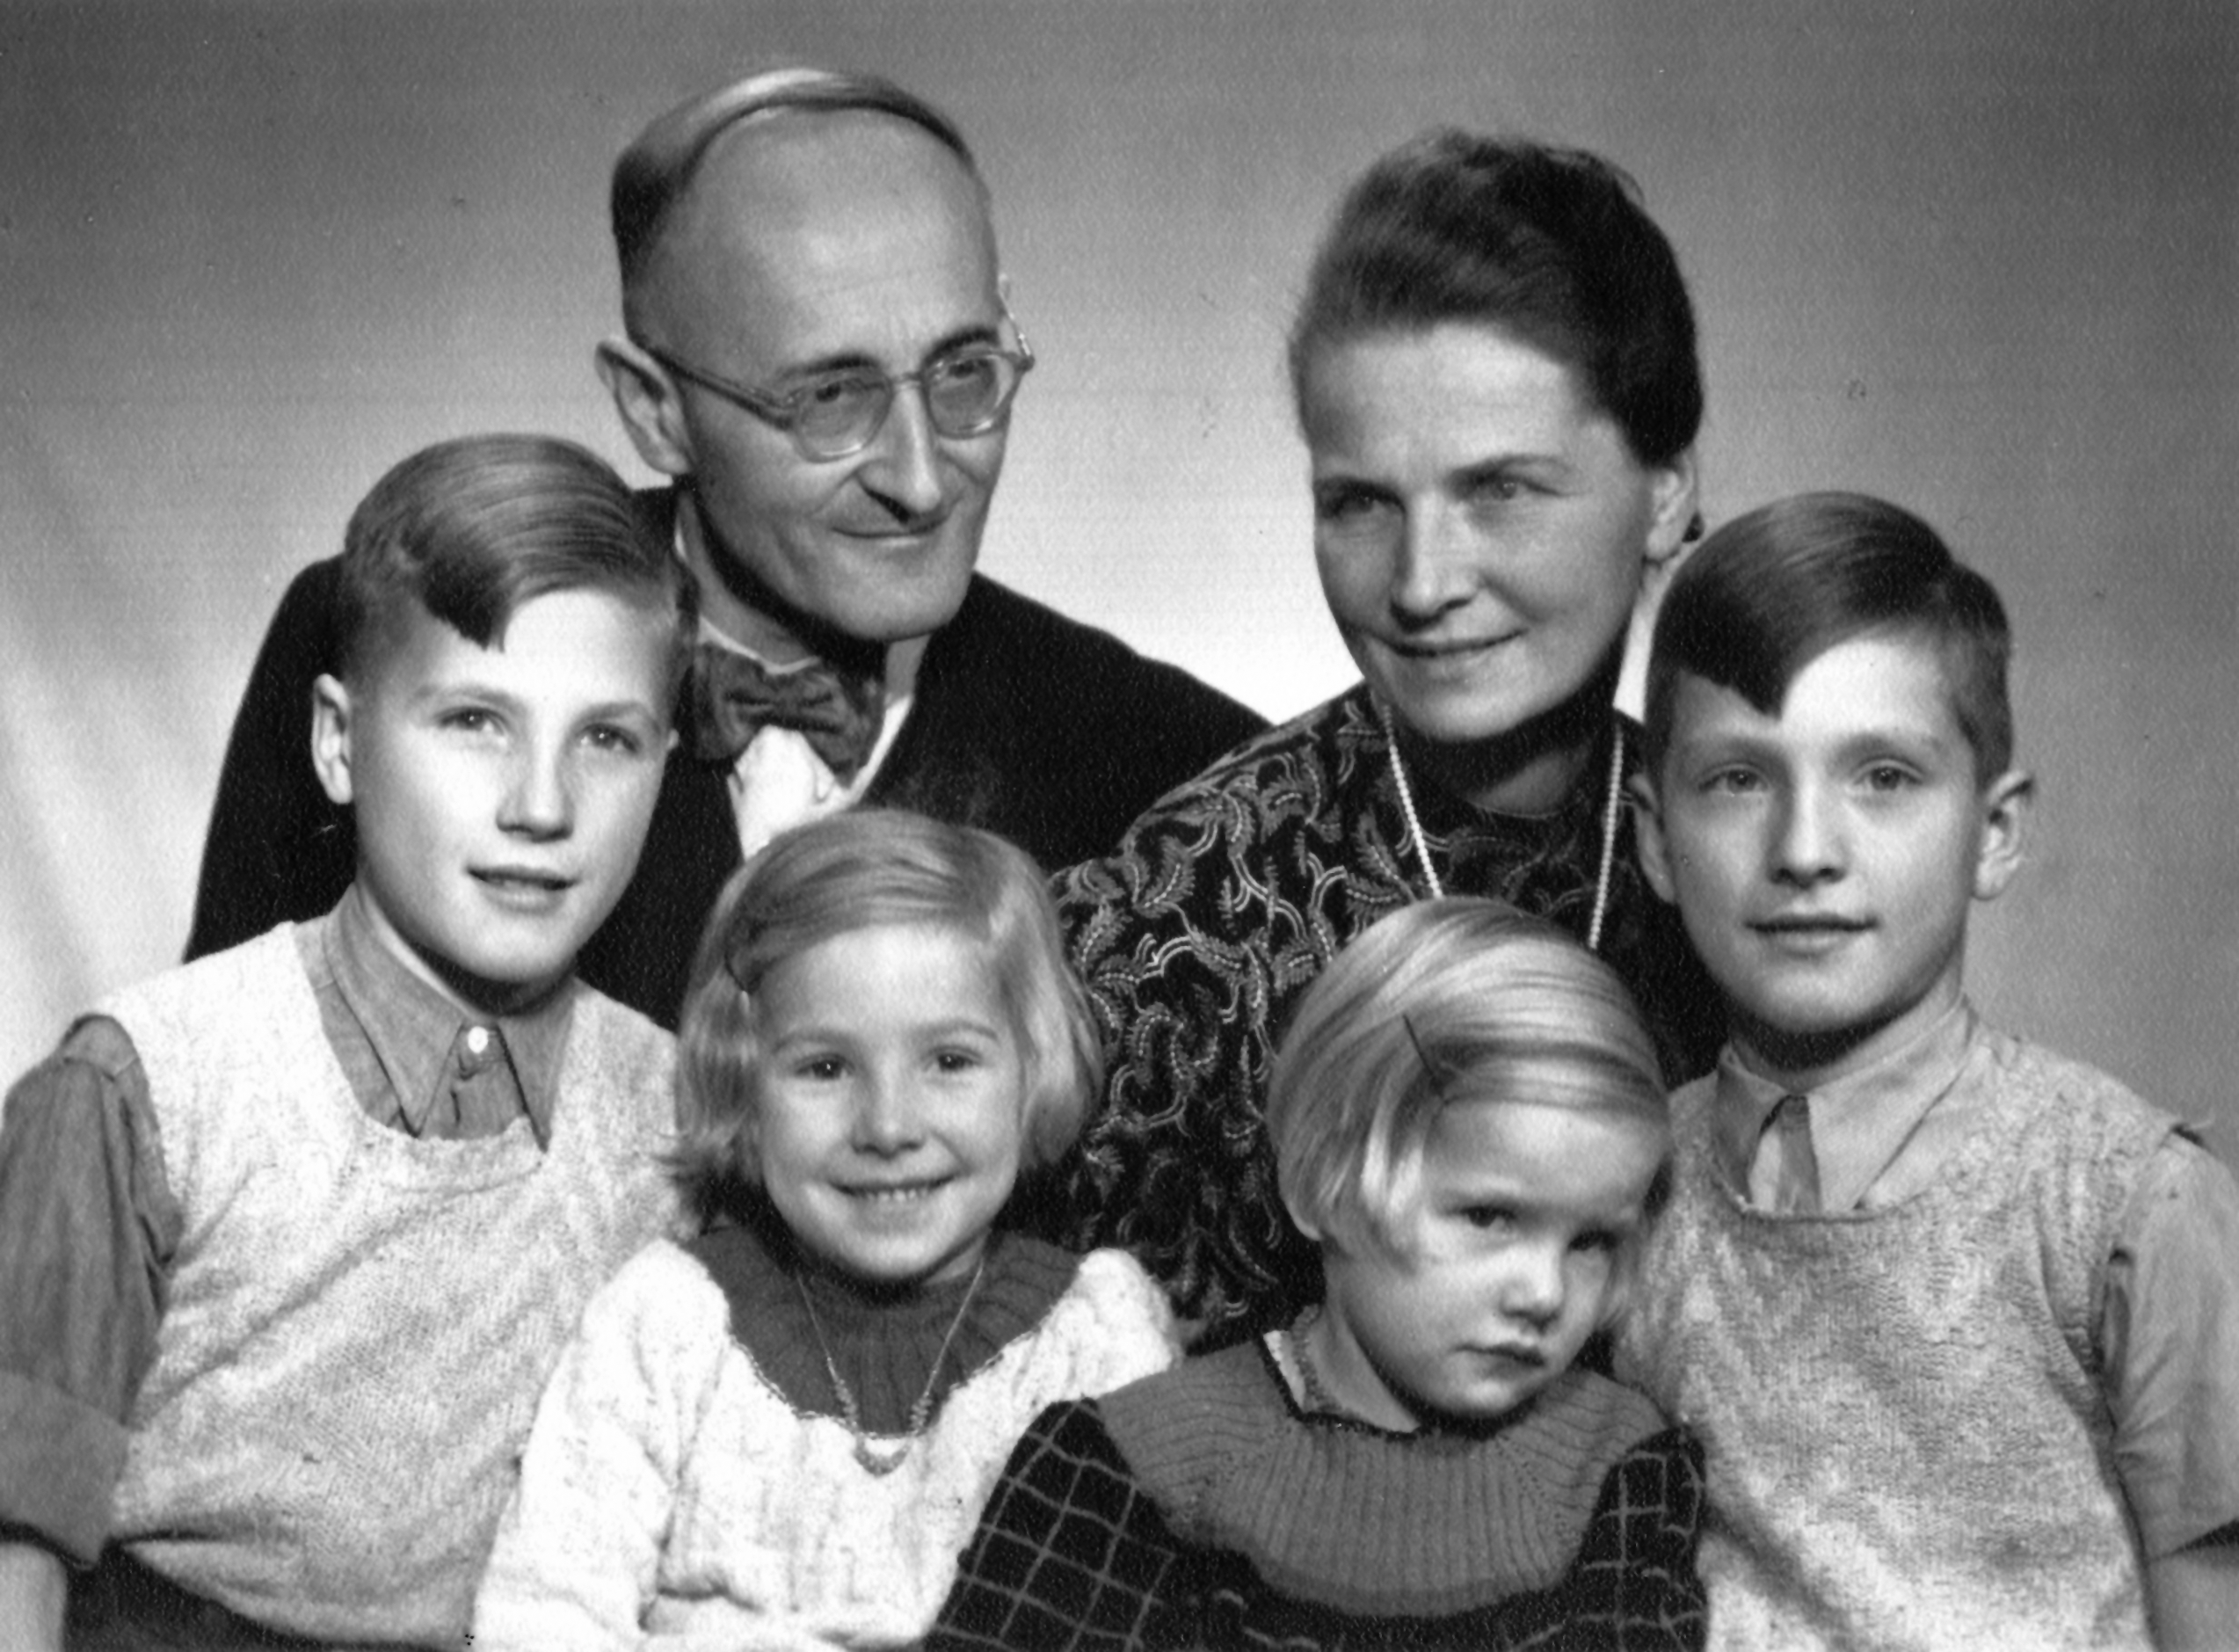
\includegraphics[width=\linewidth]{Photos/Weihnachten-1948.png}}
	\caption{Weihnachten 1948, von links nach rechts: Wolfgang, Helga, Ulla, Harald, hinten: Fritz und Margot}
	\label{fig:weihnachten_1948}
\end{figure}

Ein einschneidender administrativer Eingriff in unsere traditionelle Schulstruktur war die Kappung der vier unteren Klassen Sexta bis Untertertia. Alle Schüler mussten von jetzt ab ihrer Schulpflicht bis zum 14. Lebensjahr auf der Volksschule genügen. Bei mindestens befriedigenden Leistungen konnte der Volksschulabsolvent auf die jetzt 4-klassige Oberschule übergehen, die nach 4-jährigem Besuch -- die 13. Klasse fiel also fort -- mit der Reifeprüfung beendet wurde. Dieser Wandel wurde in Schul- und Lehrerversammlungen als große soziale Errungenschaft gefeiert. Die Schulleiter blieben zunächst noch auf ihrem Posten, wurden aber, wo das Pensionsalter annähernd erreicht war, in den Ruhestand versetzt und durch aktive Sozialisten, auch alte Mitglieder der SPD, ersetzt. So übernahm das Domgymnasium mit dem Ausscheiden des \ac{ostd} Weitz und seines Schwagers der Studienrat Scharfscher, der sofort dem Kollegium \marginpar{146} scharfe Töne im Sinne des SED-Staates anschlug und mit dem Schülerrat der neugegründeten FDJ\footnote{Freie Deutsche Jugend -- Organisation der Jungkommunisten} lange und anscheinend vertrauliche Gespräche führte, neben denen die Anliegen der Kollegen oft als zweitrangig behandelt wurden.

An die Stelle des plötzlich verstorbenen Stadtschulrates Linke trat ein linker SPD Volksschulrektor Germer, der sich wie sein Vorgänger von mir über alles, was man beim Umgang mit Russen wissen muss, unterrichten ließ. Er begann das Informationsgespräch mit der interessanten Äußerung: \enquote{die Russen sind die schwerste Enttäuschung meines Lebens}, so dass ich zum Anwalt der Russen werden musste. (Unser Freund Milleville bestätigte mir, dass Germer, den er sehr gut kannte, mir mit seinen einleitenden Worten eine Falle stellen wollte) Er bot mir am Ende der Unterredung an, Vorträge an der Volkshochschule zu übernehmen, was ich dann auch tat. Ich bot ihm übrigens an, eine Einführung in die Graphologie zu geben -- doch Schriftdeutung sei gar nicht gefragt. Eine begreifliche Entscheidung, wenn man weiß, was für zweifelhafte Gestalten bei einem Umsturz mit Erfolg nach oben drängen. Eine solche Gestalt war der von Anbeginn als Komet gefeierte Inspekteur aller Volkshochschulen und Abendgymnasien Sachsen-Anhalts, der \marginpar{147} die Leitung des neugeschaffenen Magdeburger Abendgymnasiums übernahm, an dem ich Deutsch in einer Abschlussklasse unterrichtete. Dieser Herr führte eine braune Aktentasche mit sich, die, wie er bei besonderen Gelegenheiten erklärte, das Bild seiner teuren, unvergesslichen Schwester enthalte, die von Hitlers Bluthunden grausam ermordet worden sei. Vor dem Kollegium und der gesamten Schülerschaft des Abendgymnasiums behauptete er, das Abitur zu besitzen, es aber auf ungewöhnlichem Wege erworben zu haben. Die Kursteilnehmer, Erwachsene zwischen 18 und 40 Jahren, würden zwar jetzt von Studienräten unterrichtet, die Reifeprüfung werde jedoch nicht vor Akademikern, nicht vor Männern der Theorie, sondern von solchen der Praxis, vor Werkmeistern, vor Männern mit harten Arbeitshänden abgelegt.

Sein Geburtstag wurde höchst feierlich begangen, das Podium des Festsaales war von einem Blumenmeer umgeben. Der Stadtschulrat sagte in seiner Festansprache, vom Bürgertum seien früher auf diese Weise Generäle und Feldmarschalle gefeiert worden, jetzt dagegen ehre man so wahrhaft große Männer des Volkes. Der Gefeierte schien den festlichen Aufwand als etwas Gewohntes hinzunehmen und klopfte beim Betreten des Podiums pathetisch auf die Aktentasche mit dem Bild der unvergesslichen Schwester. \marginpar{148} Eines Abends besuchten seine und meine Deutschklasse gemeinsam im Stadttheater Thomas' Stück Moral. Von seinen Schülern erfuhr ich zu meiner Verwunderung, dass er in der darauffolgenden Deutschstunde die frischen Theatereindrücke nicht zu einer Besprechung des Stückes genützt hatte. Er hospitierte zuerst in meiner Stunde, die ganz dem Stück Thomas' gewidmet war und fügte am Schluss einige überflüssige klassenkämpferische Schlagworte hinzu.

Nach 1,5 Jahren verschwand dieser gefeierte Mann plötzlich von der Bühne und landete mit seiner Sekretärin im Gefängnis. Die Überprüfung der Rechnungen hatte ergeben, dass man über \num{20000} Mark für Bücherrechnungen kassiert hatte, die meisten angeschafften Bücher aber nicht auffindbar waren. Das Geld hatte der große Mann mit seiner Sekretärin auf \enquote{Dienstreisen} verjuckst. Obendrein stellte sich heraus, dass er weder ein gültiges Abiturientenzeugnis noch überhaupt eine Schwester besaß. Als gesundheitlich schwer angeschlagener Mann kam er aus dem Gefängnis heraus, seine glanzvolle Karriere war (zunächst?) beendet. Germer starb bald darauf im Alter von 52 Jahren am Herzinfarkt. Man bereitete ihm \marginpar{149} ein fürstliches Begräbnis; ein mehrere Kilometer langer Trauerzug -- Teilnahme für alle Schulen obligatorisch -- durchzog die Stadt.

Um diese Zeit hielten die Russen die Zeit für gekommen, die leitenden Stelle mit jungen, von der SED erzogenen Kräften, hier und da auch mit Altkommunisten mittleren Alters zu besetzen. Einem etwa 40-jährigen Mann der letzten Schicht wurde das Steuer im Magdeburger Schulwesen übertragen. Herr Hillenhagen, gelernter Bergmann, stieg nach 2-jähriger Tätigkeit als Schuhmachergeselle auf den Lehrberuf um und bald -- natürlich in seiner Eigenschaft als \enquote{alter} Kommunist -- zum Schulrat in Salzwedel und schließlich zum Stadtschulrat von Magdeburg auf. Er war ein aktiver Mensch von gesundem Menschenverstand, nur fehlte es ihm an guter Schulbildung. So kam es bei ihm zu peinlichen Ausrutschern, z.B. wenn er mit englischen oder französischen Eigennamen nach deutschen Ausspracheregeln umging.

Unter meinen Kursisten der Lehrerbildungsanstalt, die zu Fachlehrern des Russischen ausgebildet wurden, befanden sich zwei Mittelschulabsolventen, die sich beide durch Fleiß, Aufnahmefähigkeit und, besonders der erste von beiden, großem Ehrgeiz auszeichneten \marginpar{150} und es in kurzer Zeit \enquote{zu etwas brachten.}

Herr Rolack, der schon eine Banklehre hinter sich hatte, versprach sich jetzt vom Lehrberuf mehr Aufstiegsmöglichkeiten. Er war zunächst in die liberal-demokratische Partei eingetreten, sattelte aber schnell auf das Erfolgsrennpferd SED um. Seinen Gesinnungswandel wusste er ungemein dramatisch darzustellen: er sei bei seinen Studien auf Karl Marx' Kapital gestoßen. Dieses Buch habe ihn von der ersten Seite an gefesselt, es sei ihm wie Schuppen von den Augen gefallen, er habe begeistert erkannt, in diesem Buch liege die reine Wissenschaft, die reine Wahrheit.

Er wusste Biemüller derart für sich einzunehmen dass dieser sich überhaupt nur noch in Superlativen über ihn äußerte und ihn mit Vertrauensbeweisen überhäufte. Im Fach Russisch waren seine Leistungen zwar befriedigend, aber er gehörte nicht zu den besten des Lehrgangs. Die schriftliche Abschlussprüfung bestand in der Nacherzählung einer leichten russischen Volkserzählung, deren Titel lautete deutsch \enquote{Würzelchen und Wipfelchen}; die russischen Entsprechungen dieser Wörter waren der Klasse unbekannt. Am Morgen des Tages der schriftlichen Prüfung betrat Direktor Biemüller das Klassenzimmer, zeigte mir und den Prüflingen \marginpar{151} vorschriftsmäßig den verschlossenen aber nicht versiegelten Briefumschlag, der die Aufgaben für die schriftliche Prüfung enthielt, öffnete ihn und übergab sie mir. Ich las zunächst den russischen Titel vor, um ihn gleich darauf mit deutscher Übersetzung an die Tafel zu schreiben. Doch Biemüller kam mir mit der Frage zuvor: Herr Rolack -- das heißt? Rolack: \enquote{Würzelchen und Wipfelchen}. Ich darauf: \enquote{diese Wörter sind bisher im Unterricht nicht vorgekommen -- also der ganzen Klasse unbekannt -- außer Herrn Rolack. Ich schreibe sie an die Tafel.} Durch diesen Vorfall war erwiesen, dass Biemüller seinem Günstling den russischen Text vorher zugänglich gemacht hatte. Keiner der beiden Delinquenten zeigten Spuren von Verlegenheit; einige Prüflinge grinsten. Rolacks Arbeit war einwandfrei gut, das Gesamturteil \enquote{mit Auszeichnung} nicht gefährdet.

Als ich 1,5 Jahre später bei passender Gelegenheit den \enquote{verdienten Lehrer des Volkes} an \enquote{Würzelchen und Wipfelchen} erinnerte, erblasste er.

Zunächst avancierte er zum Direktor des Domgymnasiums und damit zu meinem Vorgesetzten. Nicht viel später wurde eines Mittags der junge aber überragende Pädagoge von zwei Schulräten mit Gefolge feierlich vom Magdeburger Hauptbahnhof und zum Domgymnasium geleitet, wo ein Lautsprecher Einzelheiten über die Festlichkeit \marginpar{152} verkündete: Presse, Film und Rundfunk hatten sich im Domgymnasium eingefunden. Für den Film führte eine Gruppe von uns ein gestelltes pädagogisches Gespräch mit dem in Berlin zum \enquote{Verdienten Lehrer des Volkes} erhobenen Pädagogen. Er strahlte mehrere Jahre am pädagogischen Himmel. Doch sein Ehrgeiz ließ ihn nicht schlafen: er strebte noch weiter nach oben an die Pädagogische Hochschule und Universität Potsdam. Die Voraussetzung hierfür war die Vorlage einer wissenschaftlich qualifizierten Arbeit. Also verfasste er eine Dissertation, die sich leider an der Humboldt Universität als reines Plagiat erwies. Der \enquote{Verdiente Lehrer des Volkes} verlor diesen Ehrentitel und die mit ihm verbundenen finanziellen Vorteile, dazu den Direktorposten und wurde mit zweijähriger schwerer Arbeit in einem Rüstungsbetriebe bestraft. Was weiter aus ihm geworden ist, habe ich nicht erfahren können. Sic transit gloria mundi\footnote{Sic transit gloria mundi = So vergeht der Ruhm der Zeit}.\\

\begin{figure}[t]
	\fbox{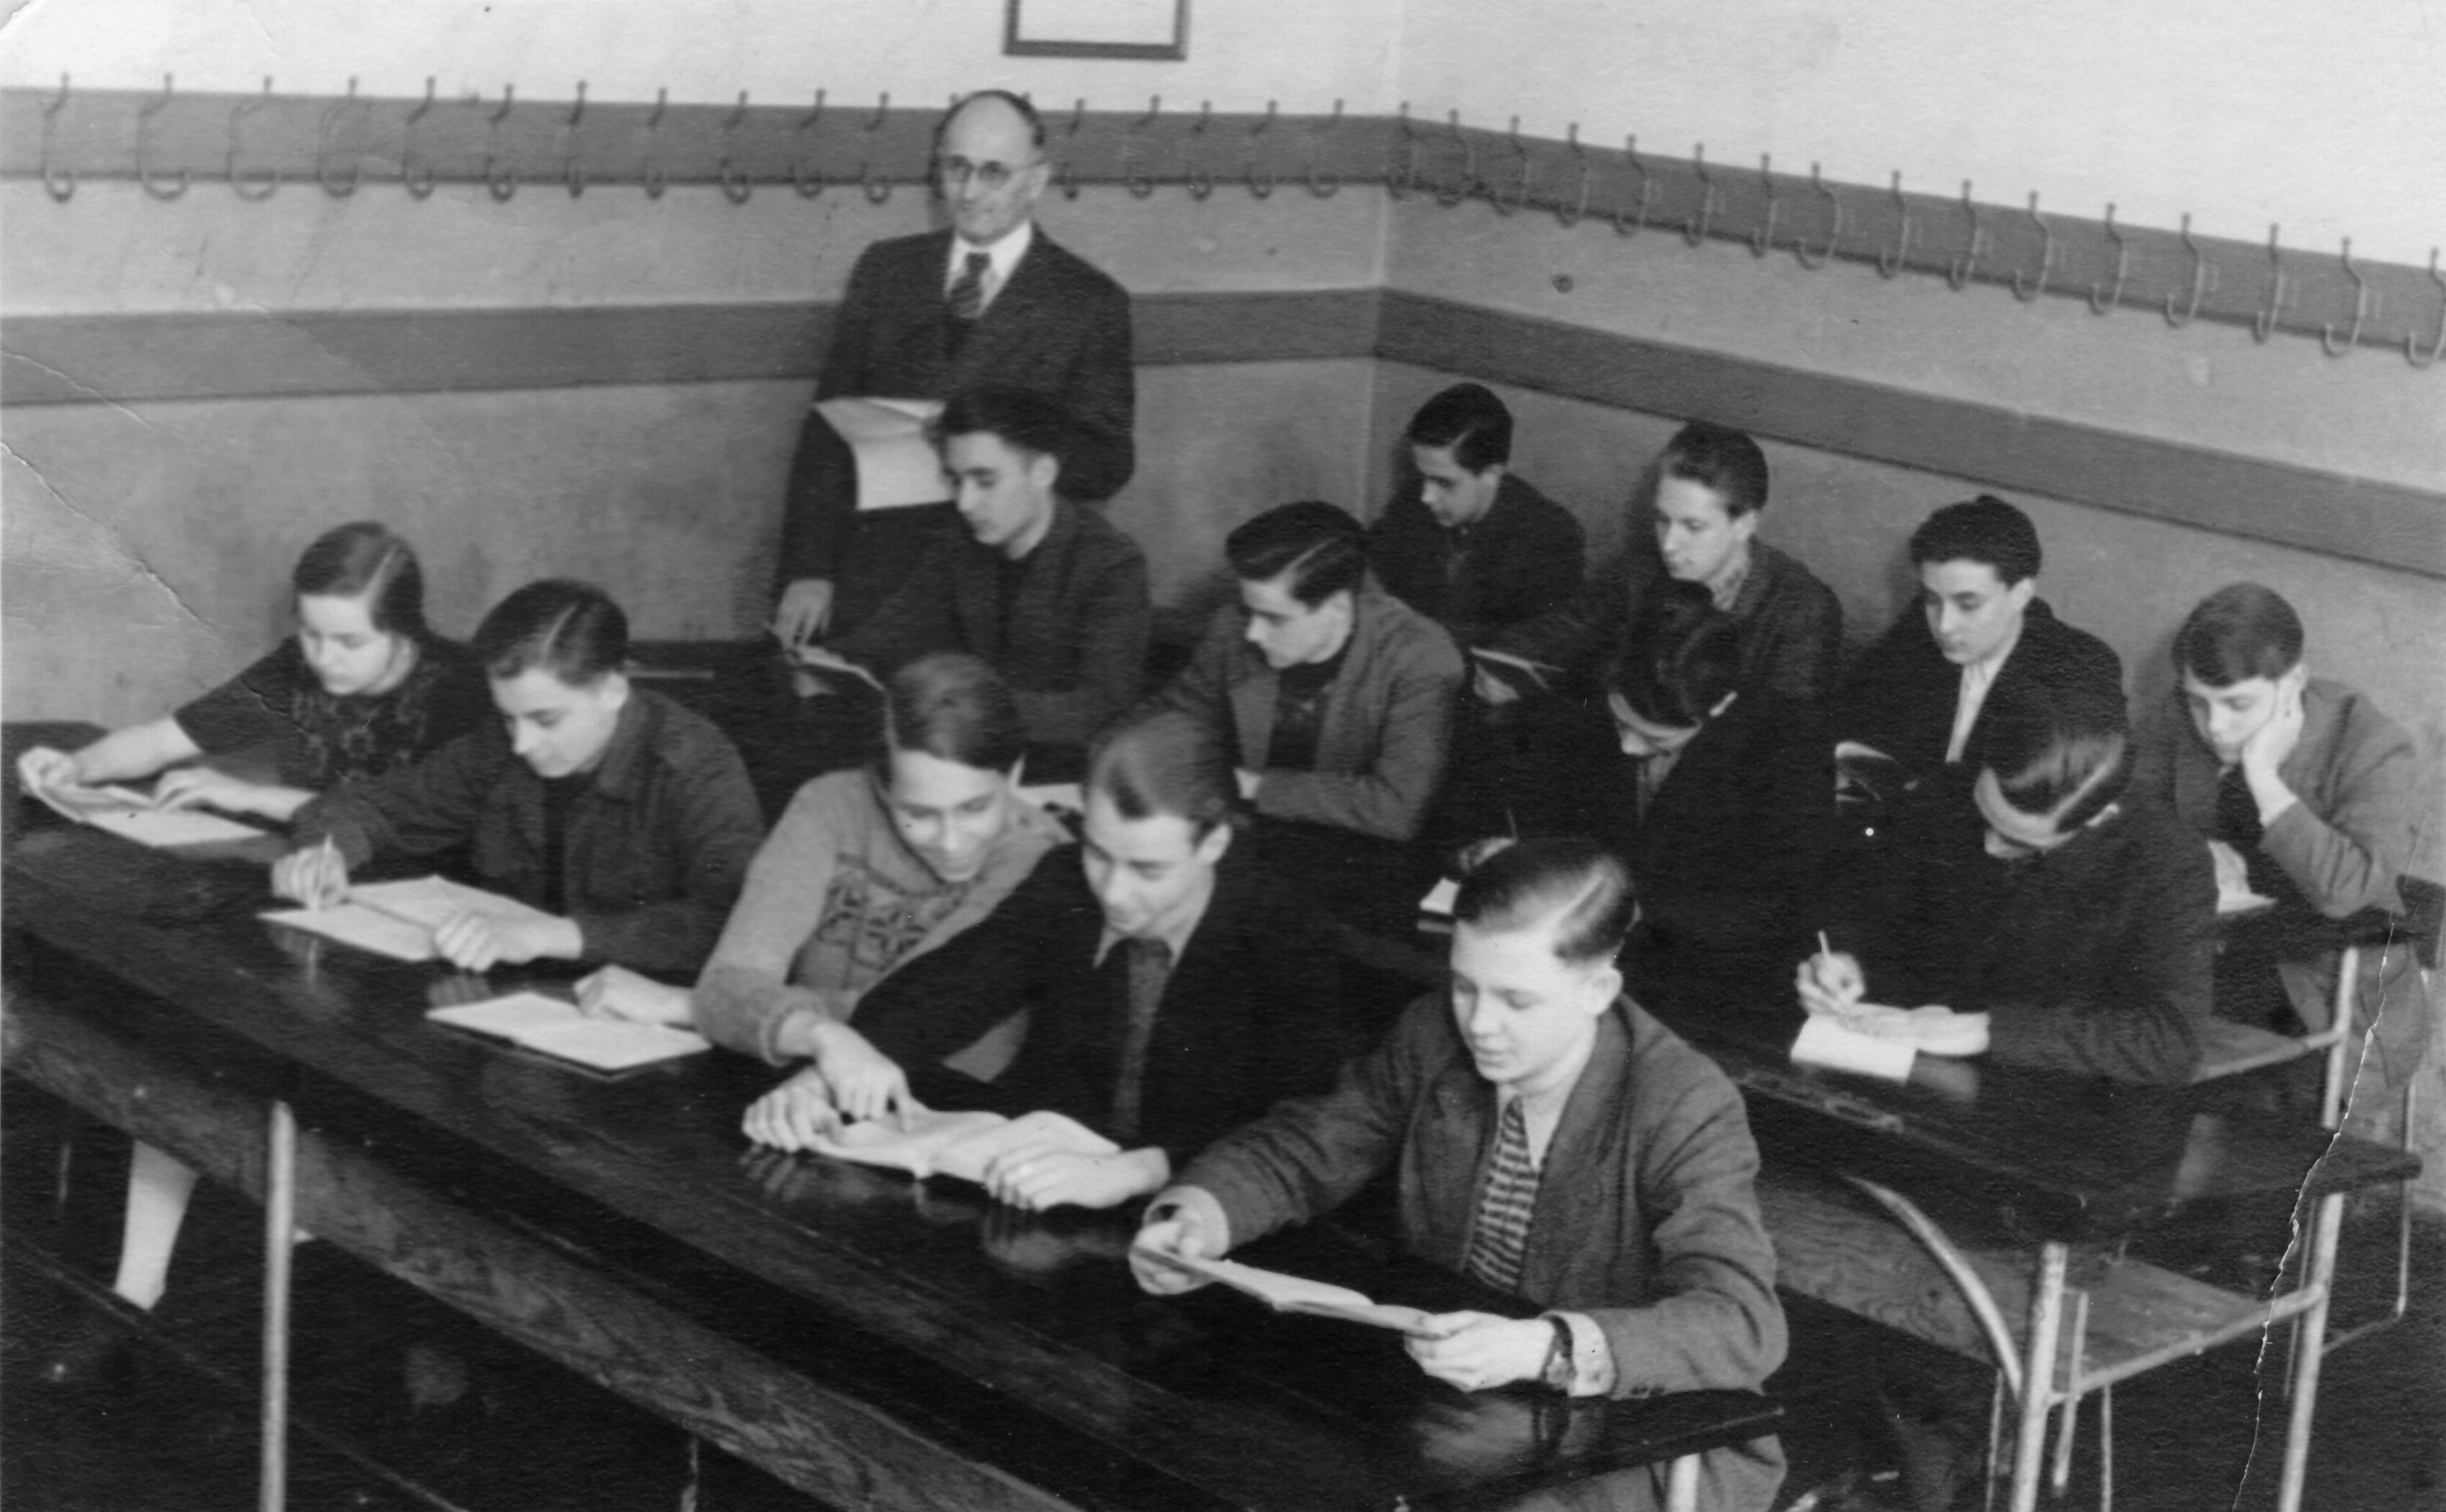
\includegraphics[width=\linewidth]{Photos/Unterricht.png}}
	\caption{Fritz während des Unterrichts, Anfang 1950er Jahre in\linebreak Magdeburg}
	\label{fig:unterricht_magdeburg}
\end{figure}

Doch damit bin ich der chronologischen Entwicklung der Ereignisse um einige Jahre vorausgeeilt, denn zur Zeit von Rolacks Sündenfall war ich längst nicht mehr in Magdeburg tätig.

Herr Rott war einer der fleißigsten und der strebsamste Fachlehrer-Aspirant seiner Russischklasse, \marginpar{153} in etwa zwei Monaten stand er vor seiner Abschlussprüfung. Seine Russischstunden plante er mit besonderer Sorgfalt, wie überhaupt der Methodik des Unterrichts sein besonderes Interesse galt. Einige Monate nach dem Amtsantritt Rolacks als Direktor des Domgymnasiums erschien er vor dem Unterricht bei mir und stellte sich als Referent des russischen Unterrichts für den Bezirk Magdeburg-Schönebeck und damit als mein Fachvorgesetzter vor. Ich war für Sekunden sprachlos, er bemerkte es und klopfte mir wohlwollend auf die Schulter mit den Worten: \enquote{So, nun setzen Sie sich erstmal hin und schlucken Sie die Kröte runter!} Ich brauchte tatsächlich einige Sekunden um Luft zu schöpfen und ihn zu seiner ungeahnten Beförderung \underline{vor} Ablegung der Fachlehrerprüfung zu gratulieren: er sei wohl jetzt in etwa den Rang eines Schulrates erhoben worden? Er bejahte meine Frage und eröffnete mir gleichzeitig, er wolle bei mir in vier Wochen die Fachlehrerprüfung in Russisch ablegen. Mit dieser Ankündigung hatte ich wieder Oberwasser und eröffnete ihm meinerseits, dass sich jetzt für ihn die Prüfungssituation grundsätzlich geändert habe; ich könne ihm in der Prüfung \marginpar{154} natürlich nicht so simple Fragen stellen wie den anderen Fachlehrer-Aspiranten, das wäre ja geradezu eine Respektlosigkeit vor der Würde seiner neuen Stellung, und ich nannte einige Gebiete und Themen aus Sprachgeschichte und Literatur, über die ich ja Vorträge gehalten hatte. Jetzt packte meinen Rott die Prüfungsfurcht, und er flehte mich an, ihm das doch nicht anzutun sondern auch ihm gegenüber bei meinen durchschnittlichen Prüfungsanforderungen zu bleiben. Doch ich ließ ihn weiter zappeln.

Im übrigen schaffte er in der Prüfung die 2 und er benahm sich in den zwei Jahren die ich noch mit ihm zu tun hatte, mir gegenüber durchaus taktvoll. Nur ein Mal erlaubte er sich die Vorzensur eines Abiturienten von \enquote{mangelhaft} in \enquote{ausreichend} heraufzusetzen und ihn damit zur Reifeprüfung zuzulassen mit der Begründung, die Leistungen meiner Schüler lägen in Russisch durchweg um eine Nummer über denen der anderen Oberschulklassen in Magdeburg, sodass Schüler, die bei mir \enquote{ausreichend} hätten, anderswo mit mindestens \enquote{befriedigend} und solche, die bei mir \enquote{mangelhaft} hätten, vergleichsweise mit \enquote{ausreichend} beurteilt würden. Und dies geschah mir mit einer Prima, in der ich drei \marginpar{155} mit 1, acht mit 2, sechs mit 3, drei mit 4 und nur einen mit 5 (mangelhaft) zensiert hatte!

Rott, der schon einige Beiträge über Methodik des Russischunterrichts, die vor allem für die unteren Klassen sehr nützlich waren, in der amtlichen Fachzeitschrift veröffentlicht hatte, erschien eines Tages bei mir mit einem umfangreichen Manuskript, einer \enquote{Methodik des Russischunterrichts}, die, wie er sagte, zu drei Vierteln fertig sei, es fehlten nur noch einige Kapitel über Phonetik, Syntax und andere linguistische und literarische Fragen, die ich bearbeiten solle. Nach eingehender Prüfung des Manuskriptes musste ich seinen Wunsch ablehnen, da die Arbeit den wissenschaftlichen Anforderungen nicht entsprach und ich keine Neigung verspürte, mich durch meine Mitarbeit zu kompromittieren. Er war betrübt, verzichtete offenbar auf seinen ehrgeizigen Plan, veröffentlichte hin und wieder einen Aufsatz über ein methodisches Problem und war, als ich ihn 1955 wiedersah, Kreisschulrat geworden.\\

\noindent\rule{12cm}{0.4pt}

\begin{addmargin}[25pt]{30pt}
\noindent Hier brechen die handschriftlichen Aufzeichnungen in der Mitte des Oktavheftes ab.
\end{addmargin}
